\section{Messung der Absorptionsschichtdicke von verschiedenen Detektoren}

\subsection{Halbleiterdetektor}

\subsubsection{Aufbau}

\begin{minipage}{0.5\textwidth}
blabla
\begin{figure}
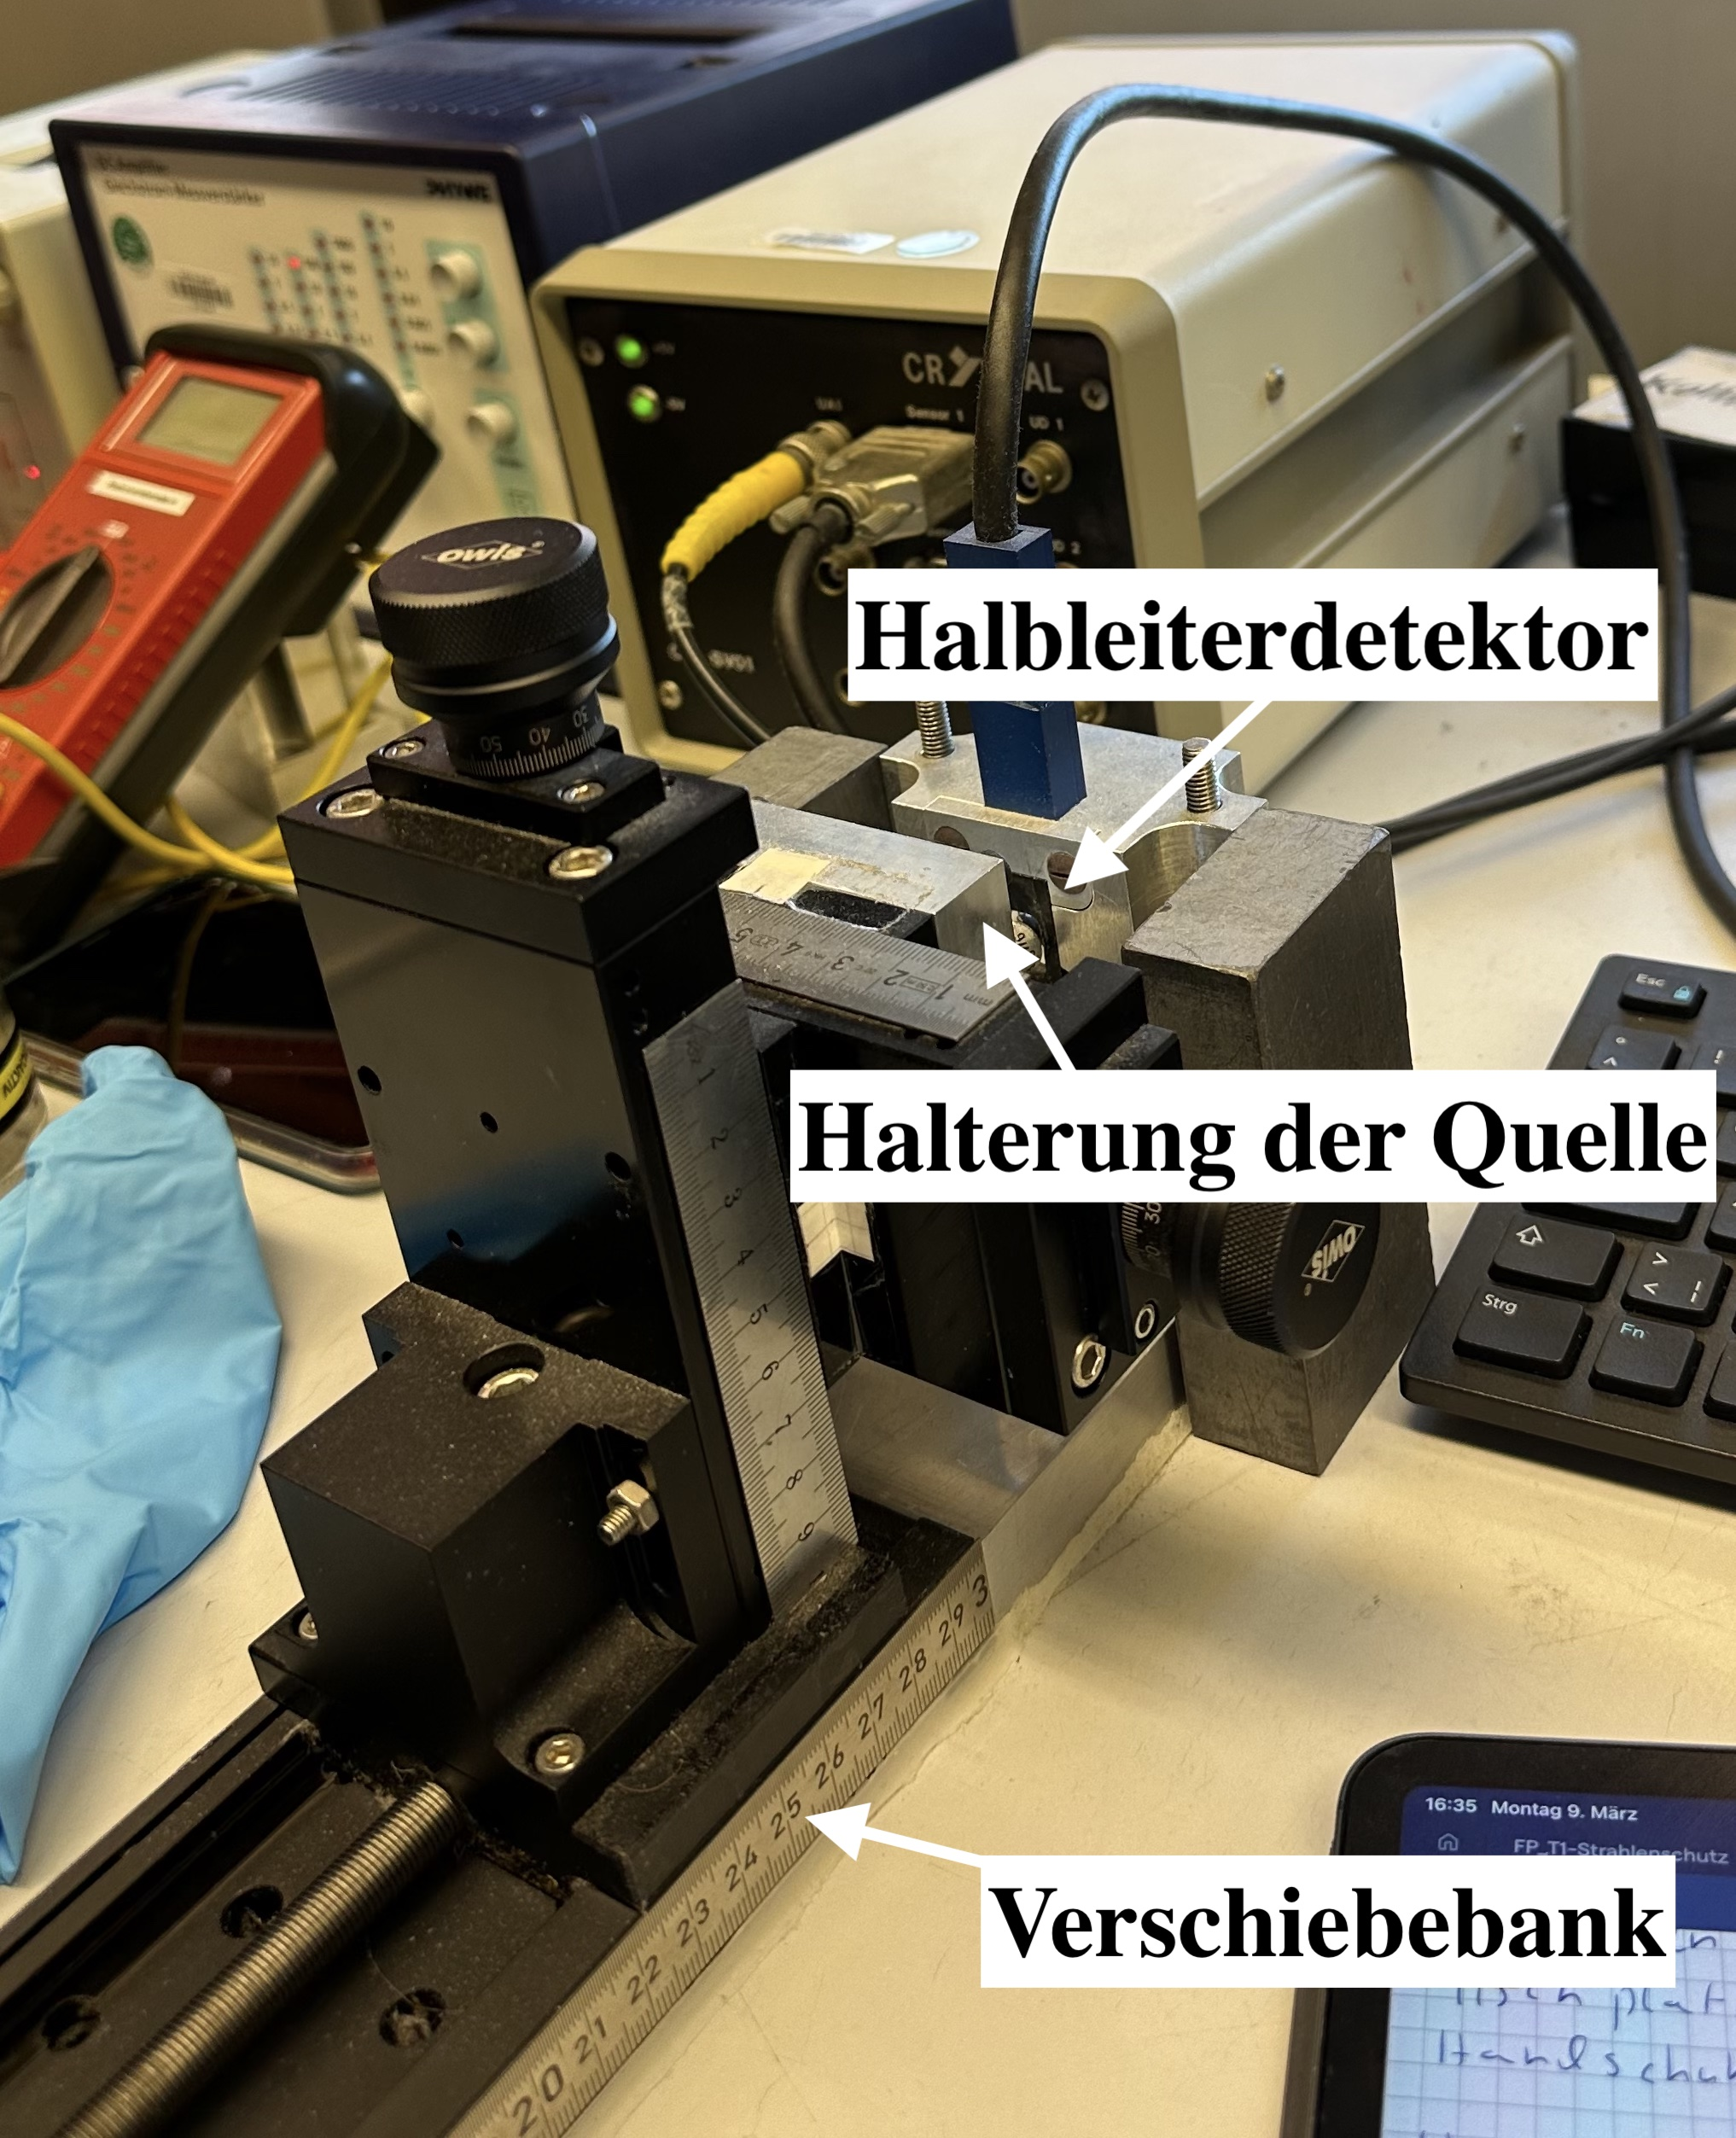
\includegraphics[width = 1\textwidth]{Bilder/Aufbau_Halbleiter.jpg}
\caption{\label{fig:Aubau_Halbleiter} Aufbau}
    \end{figure}
\end{minipage} \hfill
\begin{minipage}{0.45\textwidth}

Der Aufbau besteht aus einem Halbleiterdetektor vor dem eine $^{226}$Ra-Quelle auf einer Verschiebebank mit Lineal angebracht ist. Der Halbleiterdetektor ist über einen Verstärker und Vielkanalanalysator mit dem Computer verbunden zur Datendarstellung und -speicherung im Programm Genie 2000. 

\end{minipage}

\subsubsection{Keine Ahnung}

\begin{figure}[ht]
    \centering
    \includesvg[width=0.8\textwidth]{Bilder/Gesamtspektrum_mit_Fit.svg}
    \caption{Gesamtes aufgenommenes Spektrum mit Fit}
    \label{fig:HalbleiterSpektrumAlles}
\end{figure}



\begin{table}[H]
    \centering
    \begin{tabular}{|c|c|}
    \Xhline{1.5pt}
    \multicolumn{2}{|c|}{Ermittelte Positionen der Peaks}\\ \Xhline{1.5pt}
    Peak 1 & $2290.6\pm15.4$ \\ \hline
    Peak 2 & $3749.2\pm3.1$ \\ \hline
    Peak 3 & $5055.3\pm4.9$ \\ \hline
    Peak 4 & $7808.6\pm0.5$ \\ \Xhline{1.5pt}
    \multicolumn{2}{|c|}{$\frac{\chi^2}{N_{dof}}=\frac{57157}{8200-12}\approx6.981$}\\ \hline
    \multicolumn{2}{|c|}{$\frac{\chi^2-\bar\chi^2}{\sigma_{\chi^2}}=\frac{57157-8188}{\sqrt{2\cdot8188}}\approx383$}\\
    \hline
    \end{tabular}
    \caption{Ausgewählte Fit parameter und Güte der Anpassung}
    \label{tab:Anpassung_Halbleiter}
\end{table}



Wie man am $\chi^2$ in Tabelle \ref{tab:Anpassung_Halbleiter} erkennt ist der Fit nicht besonders gut. Das errechnete $\chi^2$ ist über 300-$\sigma$ Intervalle vom Erwartungswert entfernt. Im Residuenplot \ref{fig:HalbleiterSpektrumAlles} ist außerdem eine systematische Abweichung zwischen 6000 und 7500 erkennbar. Das könnte den schlechten Fit erklären. An den Peaks, die uns besonders interessieren, sieht der Fit allerdings Vernünftig aus. Hier streuen die residueen statistisch um Null.



\subsection{Ionisationskammer}

\subsubsection{Aufbau}

\begin{minipage}{0.5\textwidth}
\begin{figure}[H]
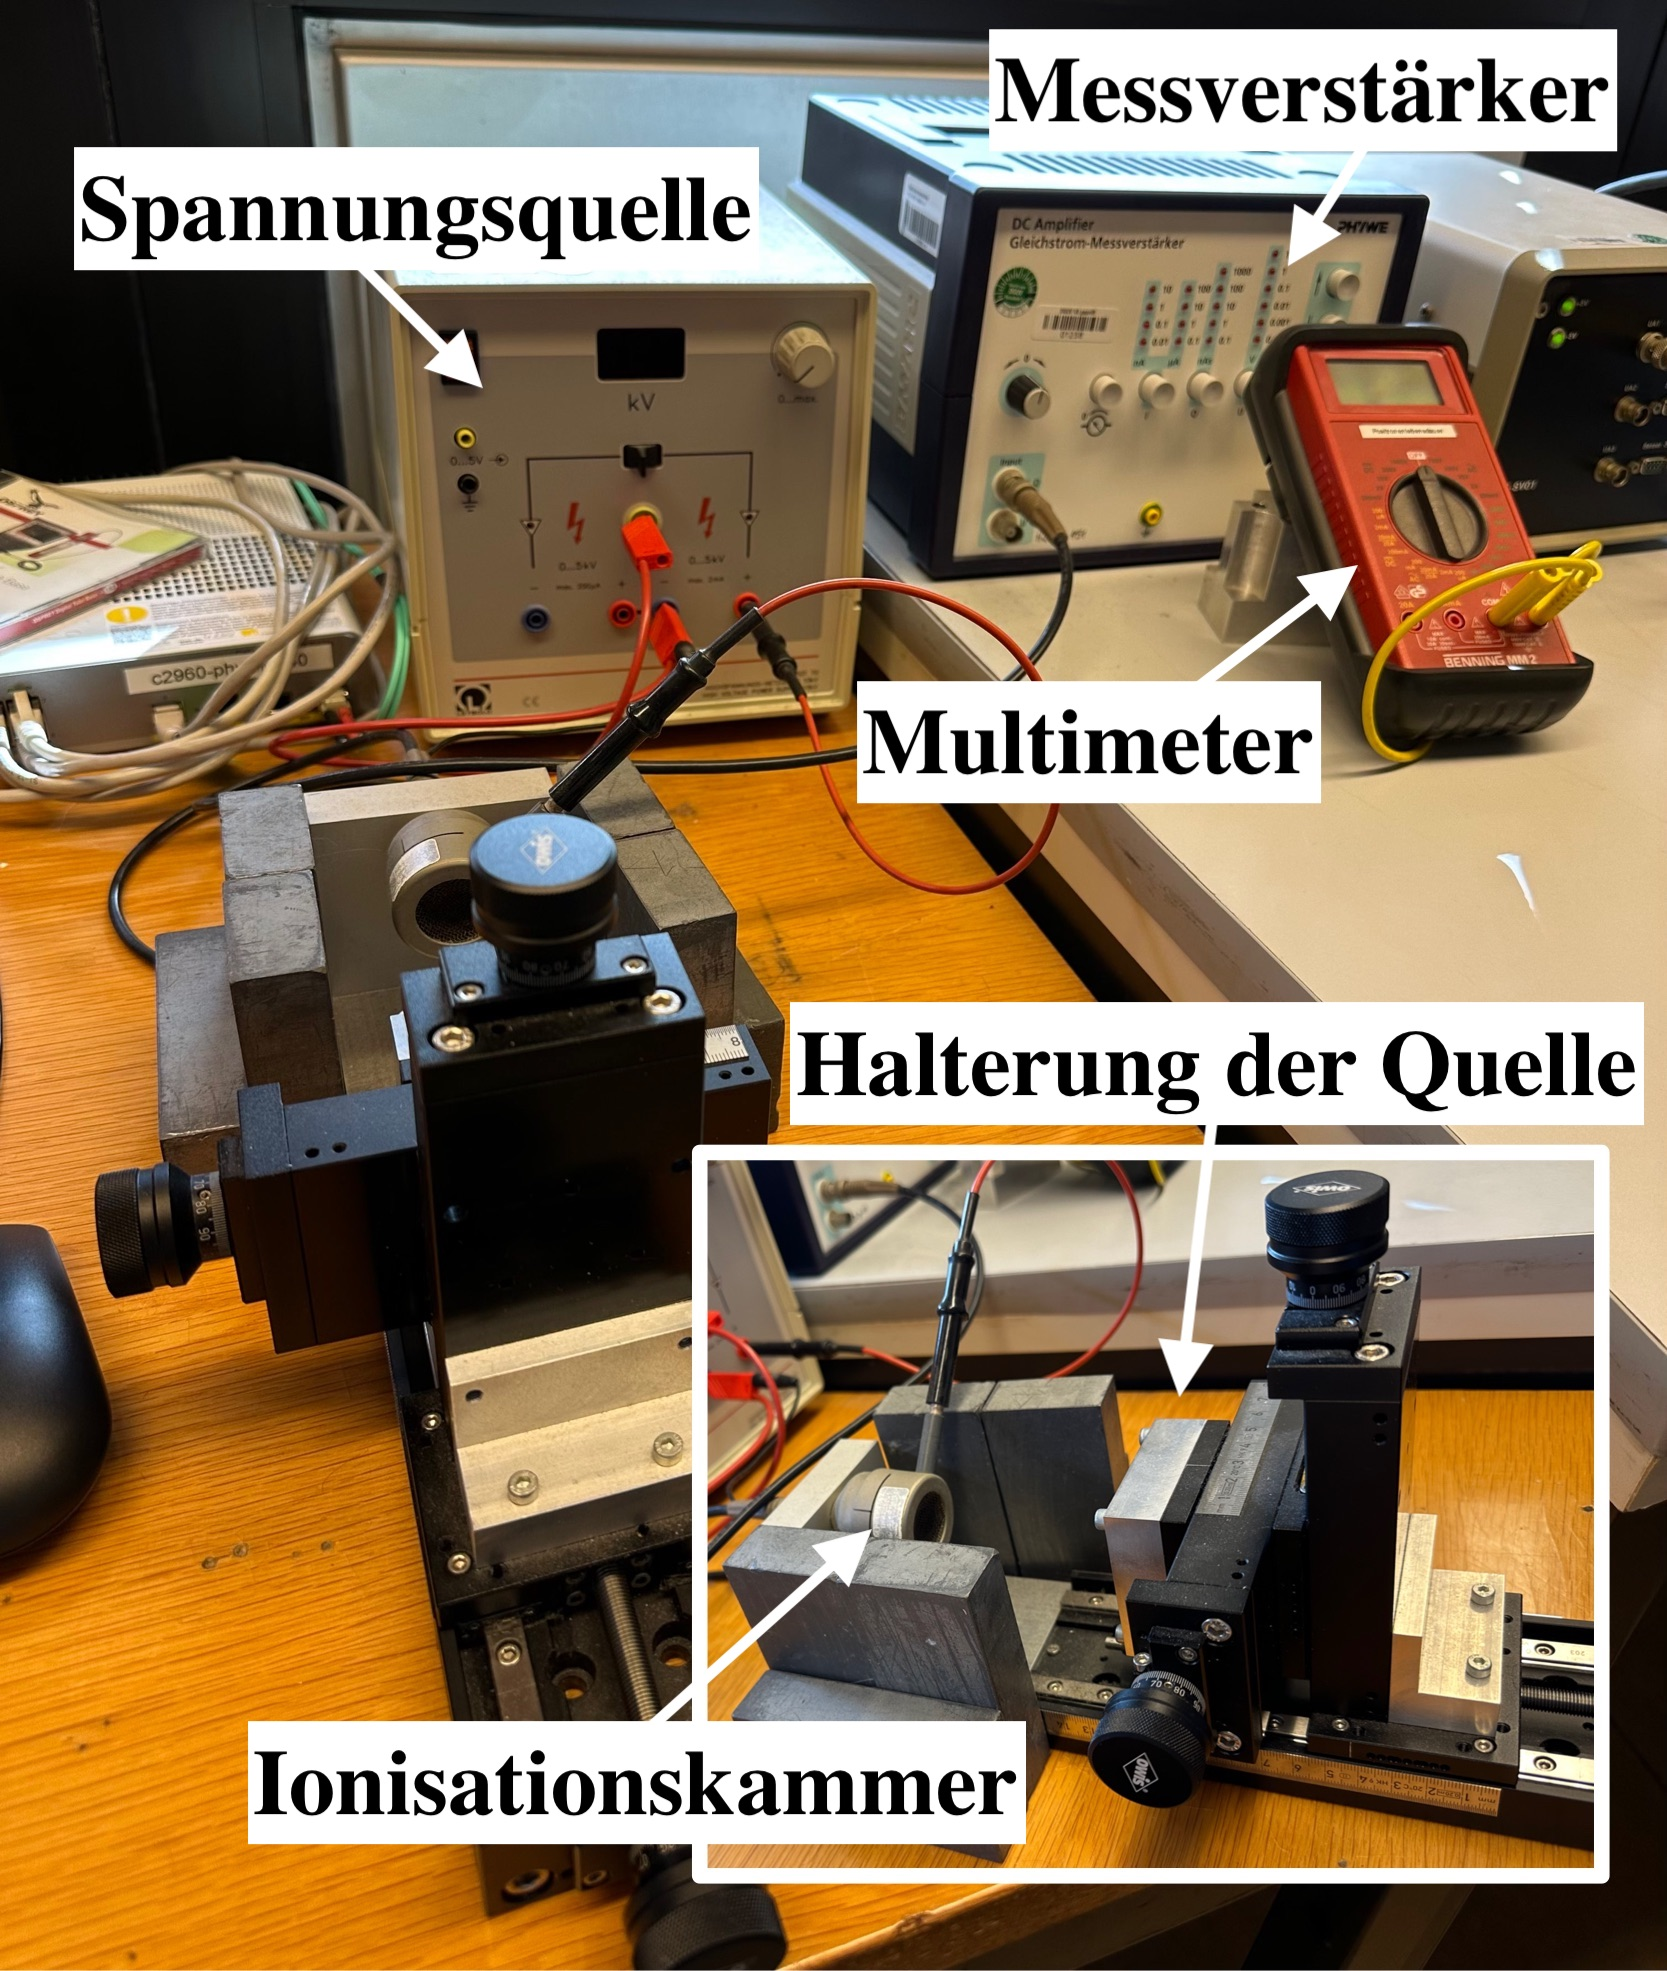
\includegraphics[width = 1\textwidth]{Bilder/Aufbau_Ionisationskammer.jpeg}
\caption{\label{fig:Aubau_Ionisationskammer} Aufbau}
    \end{figure}
\end{minipage} \hfill
\begin{minipage}{0.45\textwidth}

Der Aufbau besteht aus einer Ionisationskammer vor die, auf einer beweglichen Halterung mit Lineal, die $^{226}$Ra-Quelle angebracht ist. Das Gitter der Ionisationskammer wird über die Spannungsquelle mit Strom versorgt. Außerdem ist die Ionisationskammer mit dem Messverstärker verbunden und dieser mit dem Multimeter, um die Messwerte erfassen zu können. 

\end{minipage}


U = 1kV; Schrittweite 0.5mm aber etwas größerer Fehler da Ablesefehler; Unsicherheit bei Rauschmessung ungefähr 0.05V;
\begin{table}[H]
    \resizebox{\textwidth}{!}{
    \begin{tabular}{|l!{\vrule width 2pt}c|c|c|c|c|c|c|}
    \hline
    Abstand (\si{\cm})&$9.05$&$8.9$&$8.7$&$8.5$&$8.3$&$8.1$&$7.9$\\
    \hline
    Strom (\SI{0.1}{\nA})&$2.90\pm0.03$&$2.68\pm0.03$&$2.68\pm0.03$&$2.40\pm0.05$&$2.04\pm0.04$&$1.68\pm0.20$&$1.32\pm0.20$\\
    \Xhline{2pt}
    Abstand (\si{\cm})&$7.7$&$7.5$&$7.0$&$6.5$&$6.0$&$5.0$&$4.5$\\
    \hline
    Strom (\SI{0.1}{\nA})&$1.02\pm0.15$&$0.775\pm0.015$&$0.435\pm0.015$&$0.365\pm0.015$&$0.360\pm0.015$&$0.115\pm0.010$&$0.0125\pm0.0015$\\
    \hline
    \end{tabular}
    }
\caption{Messwerte mit statistischen Unsicherheiten aufgrund der Schwankungen des Stroms. Zu allen Unsicherheiten kommt noch ein systematischer Fehler von 3\% vom Stromverstärker \cite{HerstellerangabenStromverstärker}. Die Fehler auf die Abstände werden vernachlässigt, da bei der verwendeten Mikrometerschraube, mit einer Auflösung von \SI{50}{\micro\m} das einem relativen Fehler von $\approx \frac{\SI{50}{\micro\m}}{\SI{75000}{\micro\m}} = 0.06\%$ entspricht. Der Gesamtfehler wird also vom Strom dominiert.}
\end{table}

Die Parameter aus den Fits sind in Tabelle \ref{tab:para_fit_scz} aufgeführt.

\begin{table}[H]
    \centering
    \begin{tabular}{|c|c|c|}
        \hline
        $A$ & $\lambda$ [\si{\per\cm}] & $\frac{\chi^2}{N_{dof}}$ \\
        \hline
        $4.68\pm0.12$&$1.1567\pm0.0206$ & $\frac{2.40}{7-2}\approx 0.48$\\
        \Xhline{1.5pt}
        \multicolumn{2}{|c|}{Plateau 1} & $2.68\pm0.03$\si{\cm}\\ \hline
        \multicolumn{2}{|c|}{Plateau 2} & $0.36\pm0.01$\si{\cm}\\ \hline
        \multicolumn{2}{|c|}{$\Delta$ Plateau} & $2.32\pm0.03$\si{\cm}\\ \hline
    \end{tabular}
    \caption{Bestimmte Paramter aus dem Fit. Für die Plateaus wurd ein gewichteter Mittelwert berechnet und für den exponentiellen Anstieg wurde mit einer Funktion $f(x)=A\cdot e^{-\lambda x}$ gefitted.}
    \label{tab:para_fit_scz}
\end{table}

\begin{figure}[h]
    \centering
    \includesvg[width=0.8\textwidth]{Bilder/Absorptionskoeffizient.svg}
    \caption{Verlauf der Stroms in Abhängigkeit des Abstands}
    \label{fig:Absorpt_Blei}
\end{figure}


Die verwendete Quelle ist umschlossen von einer Abdeckfolie aus Chrom (Anhang A \cite{Versuchsanleitung}). Dadurch wird die Energie der $\alpha$-Teilchen reduziert und die Reichweite sinkt. Um zu wissen welche $\alpha$-Teilchen zu den Plateaus gehören muss man diesen Energieverlust in Chrom mitberücksichtigen. Die Stoppingpower ($\epsilon$) von Chrom ist bei den Energien von 5-7$\,\si{\MeV}$ im Bereich von 30-40$\,\si{\eV\cm^2}$ pro Atom \cite{MasstoppingpowerCr}. Mit der dichte und dicke der Abschirmung ergibt sich:
\begin{center}
    \begin{align}
        \nonumber
        \rho &= \SI{7.1}{\g\per\cm}; \quad d= 1.8\pm{0.2}\,\si{\micro\meter}\\\nonumber
        \Delta E &= \epsilon \frac{\rho \cdot Na}{M}\cdot d \approx 0.4-0.6\,\si{\MeV} \nonumber
    \end{align}
\end{center}

Damit verlieren die $\alpha$-Teilchen um die $10\%$ ihrer Energie beim Durchgang durch das Chrom. $\alpha$-Teilchen, die aus dem Zerfall von $^{214}\text{Po}$ stammen haben eine Energie von \SI{7.69}{\MeV} \cite{Versuchsanleitung}. Nach dem Durchgang von Chrom sind es dann $\approx \SI{7}{\MeV}$. Hinzu kommt der Energieverlust in Luft über einen Abstand von \SI{0.482}{\cm} (Vgl. Gleichung \ref{eq:Plateupos}). Dabei wurde der Abstand wie folgt bestimmt:
Extrapoliert man den exponentiellen Fit in Abb. \ref{fig:Absorpt_Blei} und berechnet den Schnittpunkt mit dem Plateau 1 erhählt man folgenden Abstand:
\begin{align}
    0.482 &\pm 0.025\, \si{\cm}\quad \text{für Plateau 1}\\
    2.219 &\pm 0.058\, \si{\cm}\quad \text{für Plateau 2}
    \label{eq:Plateupos}
\end{align}
Dabei wurden die Fehler über eine Monte-Carlo-Simulation geschätzt. 



\begin{equation}
    \boxed{
       n = -\frac{dE}{dx}\frac{1}{w} \quad \text{mit } w_{\text{Luft}}\approx \SI{33.7}{\eV}
    }
\end{equation}




